\documentclass{ctexbeamer}
\setbeamercolor{titlelike}{parent=structure,bg=lightgray}
\setbeamercovered{transparent}
\usefonttheme{structurebold}
\usetheme{CambridgeUS}
%\usecolortheme{rose}
%\usecolortheme{beaver}
\usecolortheme{crane}
\useoutertheme{infolines}

\usepackage{hyperref} 
\usepackage[backend=biber,style=authortitle]{biblatex}
%\usepackage[backend=bibtex,sorting=none]{biblatex}
%\addbibresource{main.bib}
%\setbeamerfont{footnote}{size=\tiny}

\renewcommand{\figurename}{Fig}

\title{CECNET2021: Use Noise Protcol Framework to build secure communication channel for IoT scenarios}

\author{Pan Lanlan (潘蓝兰) \newline  \newline abbypan@gmail.com}
\institute[China]{Guangdong OPPO Mobile Telecommunications Corp. Ltd., China}

\date{2021.08}

\begin{document}

\frame{\titlepage}

\frame{\tableofcontents}
\clearpage

\section{IoT Secure Communication}

\subsection{Main Process}
\begin{frame}
\frametitle{Main Process}

    %\begin{enumerate}
            %\item Initial
                %\begin{enumerate}
                    %\item Pairing
                    %\item Provision/Exchange Long-Term credential
                %\end{enumerate}
            %\item Communication
                %\begin{enumerate}
                    %\item Mutual-Authentication based on Long-Term credential
                    %\item Build secure communication channel
                %\end{enumerate}
    %\end{enumerate}

    \begin{figure}[H]
        \centering 
        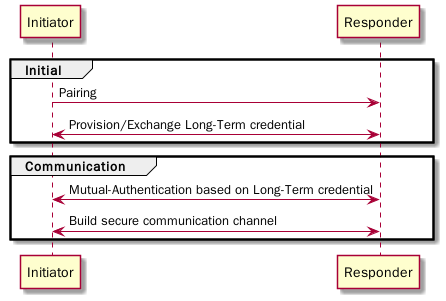
\includegraphics[width=0.7\textwidth]{pic/main_process.png} 
        \caption{Main Process} 
        \label{fig.main_process}
    \end{figure}

\end{frame}

\subsection{Initial: Pairing}
\begin{frame}
\frametitle{Initial: Pairing}

%\begin{itemize}
    %\item Balanced PAKE: Dragonfly, J-PAKE, ...
    %\item Augmented PAKE: SRP, Spake2+, ...
    %\item Other: Noise-NNpsk0, TLS-PSK, ...
%\end{itemize}

    \begin{table}[width=\textwidth]
        \begin{tabular}{ |c|l| } \hline
            \textbf{Pairing Category} & \textbf{Example} \\ \hline
            Balanced PAKE & Dragonfly, J-PAKE, ... \\ \hline
            Augmented PAKE & SRP, Spake2+, ... \\ \hline
            Other & Noise-NNpsk0, TLS-PSK, ... \\ \hline
        \end{tabular}
    \end{table}

    \end{frame}

\subsection{Initial: Provision/Exchange Long-Term credential}
\begin{frame}
\frametitle{Initial: Provision/Exchange Long-Term credential}

\begin{itemize}
    \item Share Secret
    \item Endpoint's Raw Public Key
    \item Endpoint's Certificate
\end{itemize}

    \end{frame}

\subsection{Communication: Mutual-Authentication based on Long-Term credential}
\begin{frame}
\frametitle{Communication: Mutual-Authentication based on Long-Term credential}

%\begin{itemize}
        %\item STS: Full STS, Basic STS, ...
        %\item SIGMA: SIGMA-I, SIGMA-R, ...
        %\item TLS: mutual TLS, TLS-PSK, ...
        %\item MAC: HMAC, C-MAC, ...
        %\item Noise: Noise-KK, Noise-IX, Noise-XX, ...
        %\item Other: ...
%\end{itemize}

    \begin{table}[width=\textwidth]
        \begin{tabular}{ |c|l| } \hline
            \textbf{Authentication Category} & \textbf{Example} \\ \hline
            STS & Full STS, Basic STS, ... \\ \hline
            SIGMA & SIGMA-I, SIGMA-R, ... \\ \hline
            TLS &  mutual TLS, TLS-PSK, ... \\ \hline
            MAC & HMAC, C-MAC, ... \\ \hline
            Noise & Noise-KK, Noise-IX, Noise-XX, ...  \\ \hline
            Other & ... \\ \hline
        \end{tabular}
    \end{table}

    \end{frame}

\subsection{Communication: Build secure communication channel}
\begin{frame}
\frametitle{Communication: Build secure communication channel}

\begin{itemize}
    \item Single Key: Symmetric Encryption(AEAD)
    \item Separated Keys: Symmetric Encryption + Symmetric Authentication 
\end{itemize}
    \end{frame}

\section{IoT Secure Scenario}

\subsection{Secure IoT Communication}
\begin{frame}
    \frametitle{Secure IoT Communication}
           \begin{itemize}
               \item Resource Constrained: Limited CPU/Memory/Battery
               \item Payload Size: Cut Down
               \item Compatible: Different Credentials
               \item Privacy: ID Protection
           \end{itemize}
\end{frame}

\subsection{Example: Matter}
\begin{frame}
    \frametitle{Example: Matter}

           %\begin{enumerate}
               %\item Initial Pairing: Spake2+
               %\item Provision/Exchange Long-Term credential: Endpoint's Certificate
               %\item Authentication: SIGMA-I
               %\item Communication channel: Single Key
           %\end{enumerate}

    \begin{table}[width=\textwidth]
        \begin{tabular}{ |c|l| } \hline
            \textbf{Process} & \textbf{Selection} \\ \hline
            Pairing & Spake2+  \\ \hline
            Credential & Endpoint's Certificate \\ \hline
            Authentication &  SIGMA-I \\ \hline
            Communication & Single Key \\ \hline
            \end{tabular}
            \end{table}

    \begin{figure}[H]
        \centering 
        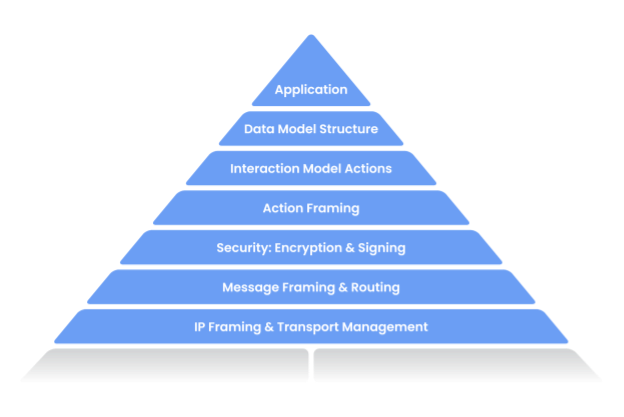
\includegraphics[width=0.5\textwidth]{pic/matter.png} 
        \caption{Matter} 
        \label{fig.matter}
    \end{figure}

\end{frame}

\subsection{Example: CCC Digital Key}
\begin{frame}
    \frametitle{Example: CCC Digital Key}

           %\begin{enumerate}
               %\item Initial Pairing: Spake2+
               %\item Provision/Exchange Long-Term credential: Endpoint's Certificate
               %\item Authentication: Vehicle signature is plaintext, Endpoint signature is encrypted.
               %\item Communication channel: Separated Keys
           %\end{enumerate}

    \begin{table}[width=0.9\textwidth]
        \begin{tabular}{ |c|l| } \hline
            \textbf{Process} & \textbf{Selection} \\ \hline
            Pairing & Spake2+  \\ \hline
            Credential & Endpoint's Certificate \\ \hline
            Authentication &  Vehicle's signature is plaintext,  \\
            ~ & Endpoint's signature is encrypted \\ \hline
            Communication & Separated Keys \\ \hline
            \end{tabular}
            \end{table}

    \begin{figure}[H]
        \centering 
        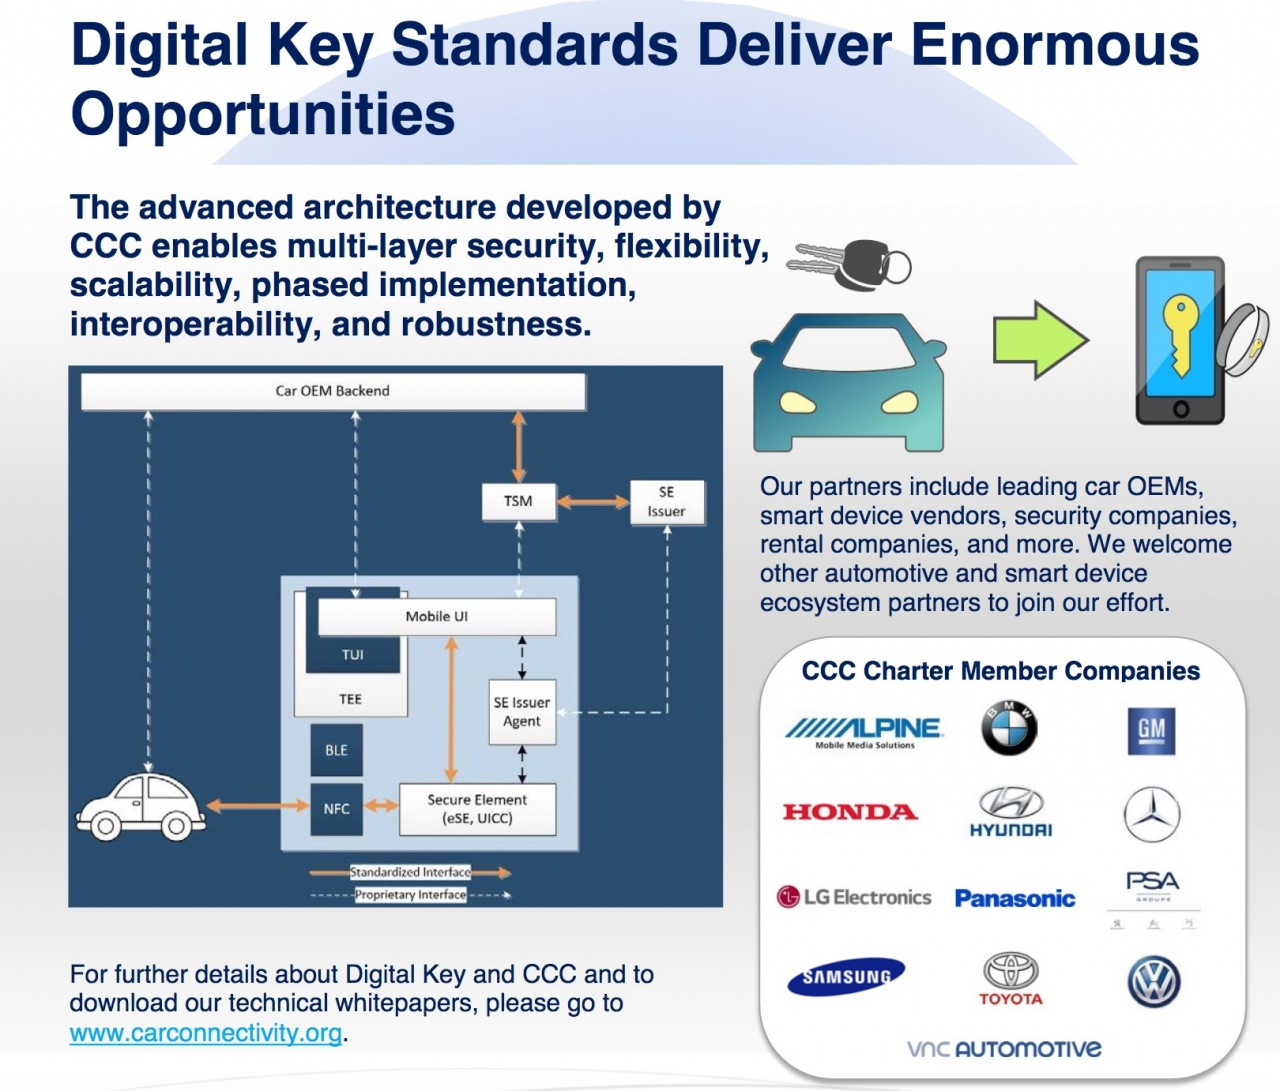
\includegraphics[width=0.35\textwidth]{pic/ccc.jpg} 
        \caption{CCC} 
        \label{fig.ccc}
    \end{figure}

    https://www.iclarified.com/66272/apple-backed-consortium-publishes-digital-key-specification-for-vehicles

\end{frame}

\subsection{Noise}
\begin{frame}
    \frametitle{Noise}

    \begin{table}[width=\textwidth]
        \begin{tabular}{ |c|l|c| } \hline
            \textbf{Pattern} & \textbf{Detail} & \textbf{Note} \\ \hline
            NNpsk0 & -> psk, e  & share secret \\
            ~ & <- e, ee, psk & simpler than balanced PAKE, TLS-PSK \\ \hline
            KK & -> s & Public Key/Certificate \\
            ~ & <- s & similar to Basic STS \\
            ~ & ... & ~ \\
            ~ & -> e, es, ss & ~ \\
            ~ & <- e, ee, se & ~ \\ \hline
            IX & -> e, s & Public Key/Certificate \\
            ~  & <- e, ee, se, s, es & Responder's ID Protection \\ 
            ~ & ~ & similar to SIGMA-R \\ \hline
            XX & -> e & Public Key/Certificate \\
            ~ & <- e, ee, s, es & Initiator's ID Protection \\
            ~ & -> s, se & similar to SIGMA-I \\ \hline
        \end{tabular}
    \end{table}

\end{frame}

\subsection{Our Proposal}
\begin{frame}
    \frametitle{Our Proposal}

    Noise: 
    \begin{itemize}
\item use DH operations to cut down the handshake signature size, which is helpful for constrained communication channel.
\item support different credentials: share secret, public key, and certificate.
\item adjust ID protection quickly by changing handshake pattern, compliance with privacy requirement, no more code development.
    \end{itemize}


    \begin{table}[width=\textwidth]
        \begin{tabular}{ |c|c|c|c| } \hline
            \textbf{Process} & \multicolumn{3}{|c|}{\textbf{Selection}}  \\ \hline
            Pairing & \multicolumn{3}{|c|}{Spake2+, Noise-NNpsk0} \\ \hline
            Credential & Share Secret & Raw Public Key & Certificate \\ \hline
            Authentication & Noise-NNpsk0 & \multicolumn{2}{|c|}{Noise-KK/IX/XX} \\ \hline
            Communication &  \multicolumn{3}{|c|}{Separated Keys} \\ \hline
        \end{tabular}
    \end{table}

\end{frame}

\section{Conclusion}

\subsection{Conclusion}

\begin{frame}
    \frametitle{Conclusion}
It is important to enhance security and privacy for IoT communication. \newline

Noise is suitable for lightweight IoT devices, compatible with different credentials, and flexible for ID protection compliance. \newline

We can use Noise Protcol Framework to build secure communication channel for IoT scenarios, compatible with various IoT Devices. \newline


    \end{frame}

\subsection{Resources}
\begin{frame}{Resources}

    \begin{thebibliography}{99}
        \bibitem{sts} STS
            https://en.wikipedia.org/wiki/Station-to-Station\_protocol

        \bibitem{matter} Matter
            https://github.com/project-chip/connectedhomeip

        \bibitem{ccc}  CCC Digital Key
            https://carconnectivity.org/

        \bibitem{noise} Noise
            https://noiseprotocol.org/

        \bibitem{sigma} SIGMA
            https://webee.technion.ac.il/~hugo/sigma-pdf.pdf

    \end{thebibliography}

\end{frame}

\end{document}
